\documentclass{beamer}
\usepackage[utf8]{inputenc}
\usepackage[brazilian]{babel}
\usepackage{pgfplots}
\usepackage{tikz}
\usepackage{amssymb}
\usepackage{mathtools}
\usepackage{array}

\usetheme{Madrid}
\usecolortheme{default}


\title{Conversão Analógica-Digital}

\author{\textbf{Pierre Machado} \and \textbf{Pedro Fernandes}}

\institute{\textbf{UEFS}}

\date{06 de Novembro de 2026}

\AtBeginSection[]
{
  \begin{frame}
    \frametitle{Sumário}\tableofcontents[currentsection]
  \end{frame}
}


% Estilos restritos às figuras e aos textos acrescentados.
\pgfplotsset{compat=1.18,pblplot/.style={width=\linewidth,height=4.3cm,
  tick label style={font=\scriptsize},label style={font=\small},
  legend style={font=\scriptsize,draw=none,fill=white},grid=major,
  scaled ticks=false,unbounded coords=jump}}
\newcommand{\pblfonte}[1]{\par\vspace{0.12cm}{\scriptsize\color{gray}Fonte: #1\par}}

% Permite quebrar os links originais sem mudar o texto das referências.
\expandafter\def\expandafter\UrlBreaks\expandafter{\UrlBreaks\do\a\do\b\do\c\do\d\do\e\do\f\do\g\do\h\do\i\do\j\do\k\do\l\do\m\do\n\do\o\do\p\do\q\do\r\do\s\do\t\do\u\do\v\do\w\do\x\do\y\do\z\do\A\do\B\do\C\do\D\do\E\do\F\do\G\do\H\do\I\do\J\do\K\do\L\do\M\do\N\do\O\do\P\do\Q\do\R\do\S\do\T\do\U\do\V\do\W\do\X\do\Y\do\Z\do\0\do\1\do\2\do\3\do\4\do\5\do\6\do\7\do\8\do\9}

\begin{document}

%The next statement creates the title page.
\frame{\titlepage}


%---------------------------------------------------------
%This block of code is for the table of contents after
%the title page
\begin{frame}
\frametitle{Sumário}
\tableofcontents
\end{frame}
%---------------------------------------------------------


\section{Introdução}
\subsection{Problema Proposto}

\begin{frame}{Problema Proposto}

\begin{columns}

    \column{0.5\textwidth}

    \begin{itemize}
        \item Compreender o processo de conversão A/D através do ATmega2560;
        \item Determinar as especificações necessárias para representar o sinal analógico, considerando as limitações do processo de conversão A/D e os erros inerentes;
        \item Avaliar os erros estáticos do conversor (offset, ganho, DNL, INL e monotonicidade) e suas características dinâmicas (faixa dinâmica, tempo de conversão e taxa máxima de amostragem).
    \end{itemize}

    \column{0.5\textwidth}

    \begin{figure}
        \centering{}
        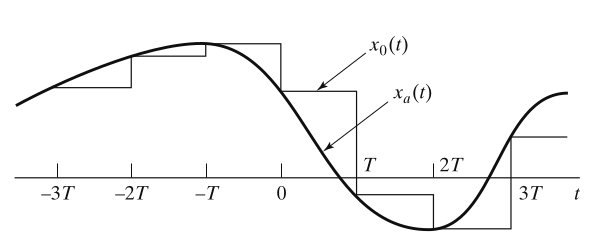
\includegraphics[width=\linewidth]{Imagens/1.png}
        \caption{Sinais de entrada e saída representativos para o sample-and-hold. Adaptado de: (Oppenheim, 2013).}
        \label{fig1}
    \end{figure}
\end{columns}

\end{frame}

\subsection{ADC e Quantização}

\begin{frame}{ADC}

    \begin{columns}
    
        \column{0.5\textwidth}
    
        \begin{itemize}
            \item O conversor analógico-digital (A/D) é um dispositivo responsável por converter sinais analógicos em representações digitais;
            \item O processo de conversão A/D é, geralmente, avaliado em três etapas:
            \begin{enumerate}
                \item Amostragem: discretização do sinal no tempo em consideração do critério de Nyquist ($f_s > 2 \cdot f_M$);
                \item Quantização: discretização do sinal na amplitude;
                \item Codificação: representação dos níveis quantizados por \textit{bits}
            \end{enumerate}
        \end{itemize}
    
        \column{0.5\textwidth}
    
        \begin{figure}
            \centering
            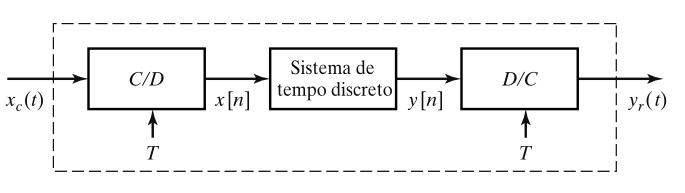
\includegraphics[width=\linewidth]{Imagens/2.png}
            \caption{Processamento em tempo discreto de sinais de tempo contínuo. Adaptado de: (Oppenheim, 2013).}
            \label{fig2}
        \end{figure}
    \end{columns}
    
\end{frame}

\begin{frame}{Quantização}

    \begin{block}{Definição}
        A quantização consiste em transformar os valores contínuos de amplitude de um sinal amostrado em um conjunto finito de níveis discretos. Os níveis, $L$, são definidos pela quantidade de \textit{bits} $N$.

        \begin{equation}
            L = 2^N
        \end{equation}

        Os níveis são utilizados para representar aproximadamente valores da tensão de referência a ser avaliada. O menor intervalo de amplitude é denominado \textbf{Least Significant Bit} (\textit{LSB}), definido da seguinte forma:

        \begin{equation}
            \Delta = \frac{V_{ref}}{L}
        \end{equation}

        Portanto, $\Delta$ é o menor incremento de amplitude que o conversor A/D consegue distinguir na escala de quantização.
    \end{block}
    
\end{frame}

\begin{frame}{Erro de Quantização}

    \begin{alertblock}{Erro de Quantização}
        Como os valores analógicos são aproximados por níveis, há erro entre o sinal original e o sinal representado, conhecido como erro de quantização, definido abaixo:

        \begin{equation}
            e_q = x - x_q
        \end{equation}

        Para quantização ideal, o erro deve ser de tal forma que o nível adotado seja o mais próximo da tensão de referência. Como a distância máxima para arrendondamento é metade do \textit{LSB}, a quantização ideal possui a seguinte faixa de erro:

        \begin{equation}
            -\frac{\Delta}{2} \leq e_q \leq \frac{\Delta}{2}
        \end{equation}
    \end{alertblock}
    
\end{frame}

\begin{frame}{Processos de Conversão A/D}

    \begin{tabular}{|>{\centering\arraybackslash}m{2.5cm}|
                >{\centering\arraybackslash}m{8.5cm}|}
        \hline
        \textbf{Método} & \textbf{Princípio de funcionamento} \\
        \hline
        \textbf{SAR} &
        Realiza comparações sucessivas entre o sinal de entrada e uma tensão de referência, determinando os bits da saída do mais significativo ao menos significativo. \\
        \hline
        \textbf{Flash} &
        Utiliza múltiplos comparadores em paralelo para comparar simultaneamente o sinal de entrada com diferentes níveis de referência. \\
        \hline
        \textbf{Sigma-Delta} &
        Utiliza sobreamostragem, integração e realimentação para realizar a conversão, empregando modelagem de ruído para aumentar a resolução. \\
        \hline
    \end{tabular}

    \begin{exampleblock}{Em relação ao Problema Proposto}
        O microcontrolador ATmega2560 utiliza o método SAR em seu conversor A/D.
    \end{exampleblock}
    
\end{frame}

\subsection{SAR}

\begin{frame}{SAR}

\begin{columns}

    \column{0.50\textwidth}

    \begin{enumerate}
        \item Sample and Hold: Captura a tensão de entrada e mantém seu valor constante durante a conversão.
        \item Comparador: Compara a tensão de entrada com a tensão de referência interna.
        \item D/A interno: Converte o código binário provisório em uma tensão analógica.
        \item Registrador SAR: Armazena e determina os bits da conversão.
        \item Controle: Coordena as etapas de comparação e atualização dos bits.
    \end{enumerate}

    \column{0.5\textwidth}

    \begin{figure}
        \centering
        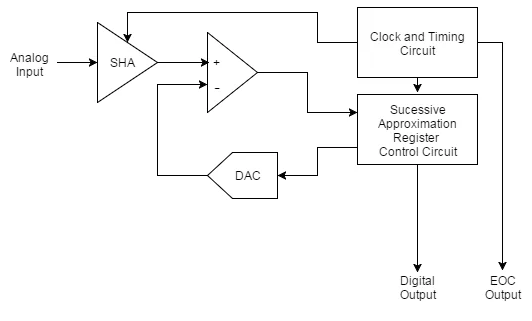
\includegraphics[width=\linewidth]{Imagens/3.png}
        \caption{Conversor A/D pelo método de Aproximações Sucessivas. Adaptado de: (Elliott Smith, 2015).}
        \label{fig3}
    \end{figure}

    
\end{columns}
    
\end{frame}

\begin{frame}{SAR: Aproximações Sucessivas}
    \begin{block}{Exemplo didático com 4 bits}
    Para $V_{in}=1{,}50$ V e $V_{ref}=2{,}56$ V:
    \begin{center}
    \small
    \begin{tabular}{ccc}
    \textbf{Código testado} & \textbf{Tensão do DAC} & \textbf{Decisão}\\\hline
    \texttt{1000} & 1,28 V & Mantém o bit\\
    \texttt{1100} & 1,92 V & Retira o bit\\
    \texttt{1010} & 1,60 V & Retira o bit\\
    \texttt{1001} & 1,44 V & Mantém o bit\\
    \end{tabular}
    \end{center}
    \end{block}
\end{frame}

\subsection{Análise Espectral: DFT e FFT}

\begin{frame}{Transformada Discreta de Fourier}

    \begin{block}{DTFS}
        Considere o sinal discreto $x[n]$ com período $N$, isto é, $x[n] = x[n + N]$. $x[n]$ pode ser representado pela série de Fourier a tempo discreto.

        \begin{equation}
            x[n] = \sum_{k=0}^{N-1} a_k e^{j\frac{2\pi}{N}kn} \;\underset{\text{Síntese}}{\overset{\text{Análise}}{\rightleftharpoons}}\; a_k = \frac{1}{N}\sum_{n=0}^{N-1}x[n]e^{-j\frac{2\pi}{N}kn}
        \end{equation}
    \end{block}

    \begin{block}{DFT}
        DFT surge a partir da DTFS quando se considera um conjunto finito de $N$ amostras de um sinal e construímos sua extensão periódica.

        Defina-se os coeficientes da DFT como $X[k]=Na_k$.
        
        \begin{equation}
            X[k]=\sum_{n=0}^{N-1}x[n]e^{-j\frac{2\pi}{N}kn}
        \end{equation}
        
    \end{block}
    
\end{frame}

\begin{frame}{Transformada Rápida de Fourier}

    \begin{block}{Algoritmo}
        A FFT é um algoritmo utilizado para calcular a DFT rapidamente. Ao avaliar a representação da DFT, é possível observar que se precisa calcular $N$ parcelas de $N$ valores possível de $k$. A complexidade algorítmica é de $O(N^2)$. Para tornar a operação mais rápida, utiliza-se a técnica de dividir e conquistar. Representa-se $X[k]$ em somatórios de índices pares e ímpares.

        \begin{equation}
            X[k] = \underbrace{\sum_{r=0}^{\frac{N}{2}-1}x[2r]e^{-j\frac{2\pi}{N}k(2r)}}_{\text{Índices pares}} + \underbrace{\sum_{r=0}^{\frac{N}{2}-1}x[2r+1]e^{-j\frac{2\pi}{N}k(2r+1)}}_{\text{Índices ímpares}}
        \end{equation}

        Repete-se o processo. Por relação de recorrência, a complexidade algorítmica é reduzida para $O(N \cdot \log_2(N))$.
    \end{block}
    
\end{frame}

\begin{frame}{Resolução Adotada}
\begin{block}{Critério de projeto}
Adota-se o fundo de escala como referência para o erro percentual.
Com 8 bits, temos 256 níveis e, para $V_{ref}=2{,}56$ V:
\[
\Delta=\frac{2{,}56}{256}=10\ \text{mV},\qquad
\frac{\Delta}{V_{ref}}\,100\%=0{,}390625\%.
\]
\end{block}
\begin{itemize}
\item Um degrau corresponde a aproximadamente $0{,}39\%$ da escala.
\item No modelo ideal com arredondamento, o erro máximo é meio LSB: $\pm 0{,}1953\%$.
\item Lê-se os 8 bits mais significativos do ADC de 10 bits.
\end{itemize}
\end{frame}

\section{Desenvolvimento}

\subsection{Avaliação Dinâmica}

\begin{frame}{Faixa Dinâmica}
\begin{block}{Faixa de entrada}
A faixa de entrada é o intervalo de tensões que o ADC pode converter sem saturar. O limite inferior é o GND e o superior é a tensão de referência:
\[
V_{\text{faixa}} = V_{\max} - V_{\min}
                = V_{\text{ref}} - V_{\text{GND}}
                = 2{,}56 - 0
                = 2{,}56\ \text{V}.
\]
\end{block}
\begin{itemize}
\item Com 8 bits, há $2^8=256$ níveis, portanto a resolução ideal é $2{,}56/256=0{,}01$ V, ou $10$ mV por LSB.
\item O código varia de 0 a 255 ao longo dessa faixa de entrada.
\end{itemize}
\begin{alertblock}{Observação}
O valor de $2{,}56$ V descreve a amplitude da faixa de entrada. Uma faixa dinâmica expressa em dB também depende do menor sinal distinguível (por exemplo, do piso de ruído); ela não pode ser calculada usando $0$ V como denominador.
\end{alertblock}
    
\end{frame}

\subsection{Captação e Transferência de Dados}

\begin{frame}{Arquitetura e Registradores}
\footnotesize
\begin{tabular}{>{\raggedright\arraybackslash}p{0.30\linewidth}p{0.62\linewidth}}
\hline
\textbf{Parte / Registradores} & \textbf{Configuração adotada} \\\hline
Entrada (\texttt{DIDR0}) & Sinal no pino A0 (\texttt{ADC0}/GND); buffer digital desabilitado. \\[0.08cm]
\texttt{ADMUX} & Referência interna de 2,56 V, canal \texttt{ADC0} e ajuste à esquerda (\texttt{ADLAR=1}). \\[0.08cm]
\texttt{ADCSRA / ADCH} & ADC habilitado, prescaler 16 ($f_{ADC}=1\text{ MHz}$) e leitura de 8 bits em \texttt{ADCH}. \\[0.08cm]
Timer1 (\texttt{TCCR1B}, \texttt{OCR1A}, \texttt{TIMSK1}) & Modo CTC com prescaler 8 ($0{,}5\ \mu\text{s}$/tick). Define $f_s$: a ISR executa \texttt{ADC\_Read()} e grava na RAM. \\[0.08cm]
UART0 (\texttt{UCSR0A/B/C}, \texttt{UBRR0}, \texttt{UDR0}) & Modo 8N1, \texttt{U2X0=1} ($\texttt{UBRR0}=16 \Rightarrow 115200$ baud), envio/recepção por \textit{polling} em \texttt{UDR0}. \\[0.08cm]
Memória (SRAM) & Buffer de $N=4096$ bytes (suporta até 6144 bytes dos 8 KB). \\\hline
\end{tabular}
\begin{exampleblock}{Aquisição em bloco (\textit{Store-and-Forward})}
Durante a coleta das 4096 amostras em RAM, a UART permanece inativa. A transmissão serial só inicia após o término da captura e parada do Timer1.
\end{exampleblock}
\end{frame}

\begin{frame}{Tempo de Conversão}
\begin{block}{Configuração utilizada}
\[
f_{ADC}=\frac{16\ \text{MHz}}{16}=1\ \text{MHz}
\]
\[
T_{conv}=\frac{13}{f_{ADC}}=13\ \mu\text{s}
\]
\end{block}
\begin{alertblock}{Condição de operação}
O datasheet recomenda 50 a 200 kHz para a resolução completa de 10 bits. Para resolução de 8 bits, admite clock de até 1 MHz.
\end{alertblock}
\begin{itemize}
\item A primeira conversão exige 25 ciclos.
\item O firmware descarta 16 leituras na inicialização e após mudar o prescaler.
\end{itemize}
    
\end{frame}

\begin{frame}{Taxa de Amostragem Máxima}
\begin{block}{Limite teórico do hardware ADC ($f_{ADC} = 1\text{ MHz}$)}
Considerando apenas a conversão ($T_{conv} = 13\ \mu\text{s}$): $f_{s,\text{ADC}} = 1 / 13\ \mu\text{s} \approx \mathbf{76{,}92\text{ kHz}}$.
\end{block}

\begin{block}{Limite operacional do firmware (leitura bloqueante na ISR)}
A ISR do Timer1 executa \texttt{ADC\_Read()} e armazena a amostra em RAM no mesmo período:
\[
C_{req} = \underbrace{14}_{\text{ciclos ADC}} \cdot \underbrace{16}_{\text{prescaler}} + \underbrace{256}_{\text{margem ISR}} = 480\ \text{ciclos de CPU } (30\ \mu\text{s}).
\]
Com Timer1 em prescaler 8 ($0{,}5\ \mu\text{s}$/tick) e $8 \cdot \text{ticks} > 480$ ($\text{ticks}_{\min} = 61$):
\[
T_{s,\min} = 30{,}5\ \mu\text{s} \implies \boxed{f_{s,\max} = 32\,786{,}9\ \text{Hz}}.
\]
\end{block}
\end{frame}

\begin{frame}{Amostragem da Onda Triangular}
\begin{block}{Quantidade de pontos por período e frequência máxima}
Para percorrer 256 níveis na subida e na descida ($512$ pontos/período):
\[
f_s \geq 2^{N_{bits}+1} \cdot f = 512 \cdot f \implies f_{\max} = \frac{f_s}{512}.
\]
\begin{itemize}
\item Para $f_{s,\text{ADC}} \approx 76{,}92\text{ kHz}$: $f_{\max} = 76\,923{,}1 / 512 \approx \mathbf{150{,}24\text{ Hz}}$.
\item Para $f_{s,\max} = 32\,786{,}9\text{ Hz}$: $f_{\max} = 32\,786{,}9 / 512 \approx \mathbf{64{,}04\text{ Hz}}$.
\end{itemize}
\end{block}
\begin{itemize}
\item Com $N_{amostras}=4096$, um ciclo requer $f \geq \frac{f_s}{4096}$.
\item Em $f_{s,\max} = 32\,786{,}9\text{ Hz}$, a faixa útil é aproximadamente \textbf{8 a 64 Hz}.
\item Em uma captura de $60\text{ Hz}$ ($60{,}49\text{ Hz}$): \textbf{542,0 amostras/ciclo}.
\end{itemize}
\end{frame}

\begin{frame}{Contraexemplos: Quantidade de Amostras}
\begin{block}{Poucos pontos por rampa ($f_s / f < 512\text{ amostras/ciclo}$)}
\footnotesize
\begin{itemize}
\item \textbf{Para $f \approx 5\text{ Hz}$, $f_s = 2048\text{ Hz}$:} obtêm-se $\approx 397\text{ amostras/ciclo}$ ($\approx 198$ pontos por rampa para $256$ níveis, violando $f_{\max} = f_s/512 = 4\text{ Hz}$);
\item \textbf{Efeito:} cada subida ou descida salta códigos individualmente; o histograma acumulado só visita os $256$ níveis por somar $10$ ciclos com fases distintas.
\end{itemize}
\end{block}
\vspace{-0.08cm}
\begin{block}{Janela menor que um período ($N_{amostras} = 4096 < f_s / f$)}
\footnotesize
\begin{itemize}
\item \textbf{Para $f \approx 1\text{ Hz}$, $f_s = 8196{,}7\text{ Hz}$:} as $4096$ amostras cobrem apenas $T_{\text{janela}} = 0{,}5\text{ s}$ (meio período, violando $f_{\min} = f_s/4096 = 2\text{ Hz}$);
\item \textbf{Efeito:} a rampa é truncada antes do pico, convertendo apenas os códigos de $0$ a $207$ e inviabilizando a caracterização de fundo de escala e FFT.
\end{itemize}
\end{block}
\vspace{-0.08cm}
\begin{exampleblock}{Compromisso na escolha de $f_s$ (buffer fixo $N = 4096$)}
\footnotesize
Para varrer os $256$ níveis por rampa e capturar ao menos $1$ ciclo completo na janela:
\vspace{-0.18cm}
\[
\frac{f_s}{4096} \le f \le \frac{f_s}{512} \quad\Longleftrightarrow\quad \boxed{512 \le \frac{f_s}{f} \le 4096\ \text{amostras/ciclo}}.
\]
\vspace{-0.28cm}
\end{exampleblock}
\end{frame}

\begin{frame}{Transferência USB e UART}
\begin{enumerate}
\item \textbf{Configuração (PC $\to$ UART):} envio de 5 bytes (prescaler, $f_s$ e $N=4096$).
\item \textbf{Captura isolada (UART inativa):} a UART fica sem transmitir enquanto a ISR do Timer1 preenche o buffer com as 4096 amostras em RAM.
\item \textbf{Envio em lote (UART $\to$ PC):} após encher o buffer e parar o Timer1, envia 1 byte de status e os 4096 bytes via UART0 (8N1, 115200 baud).
\end{enumerate}
\begin{block}{Custo da transmissão após a captura}
Cada amostra ocupa 1 byte, mas usa 10 bits no enlace ($86{,}8\ \mu\text{s}$/amostra):
\[
T_{envio}\approx\frac{4096\cdot10}{115200}=356\ \text{ms}.
\]
\end{block}
\small Em \texttt{U2X0=1}, o divisor inteiro gera $\approx 117\,647$ baud. Sem o buffer em RAM, a UART limitaria a taxa de amostragem a $\approx 11{,}5\text{ kHz}$ ($115200/10$).
\end{frame}

\subsection{Pós-Aquisição e Análise}

\begin{frame}{Tratamento no GNU Octave}
\begin{enumerate}
\item Recebe-se o bloco, verifica-se o status e as amostras são salvas em \texttt{.mat}.
\item Estima-se período e fase para alinhar a triangular simulada ao sinal capturado.
\item Compara-se a referência contínua, a versão quantizada e os códigos do ADC.
\item São calculados os erros no tempo, o histograma de códigos e os espectros.
\end{enumerate}
\begin{block}{Comparação utilizada}
O erro bruto compara os códigos com a triangular ideal de 0 a 255. O erro residual remove ganho e offset ajustados.
\end{block}
\end{frame}

\begin{frame}{Painel do Analisador no GNU Octave ($10\text{ Hz}$)}
\centering
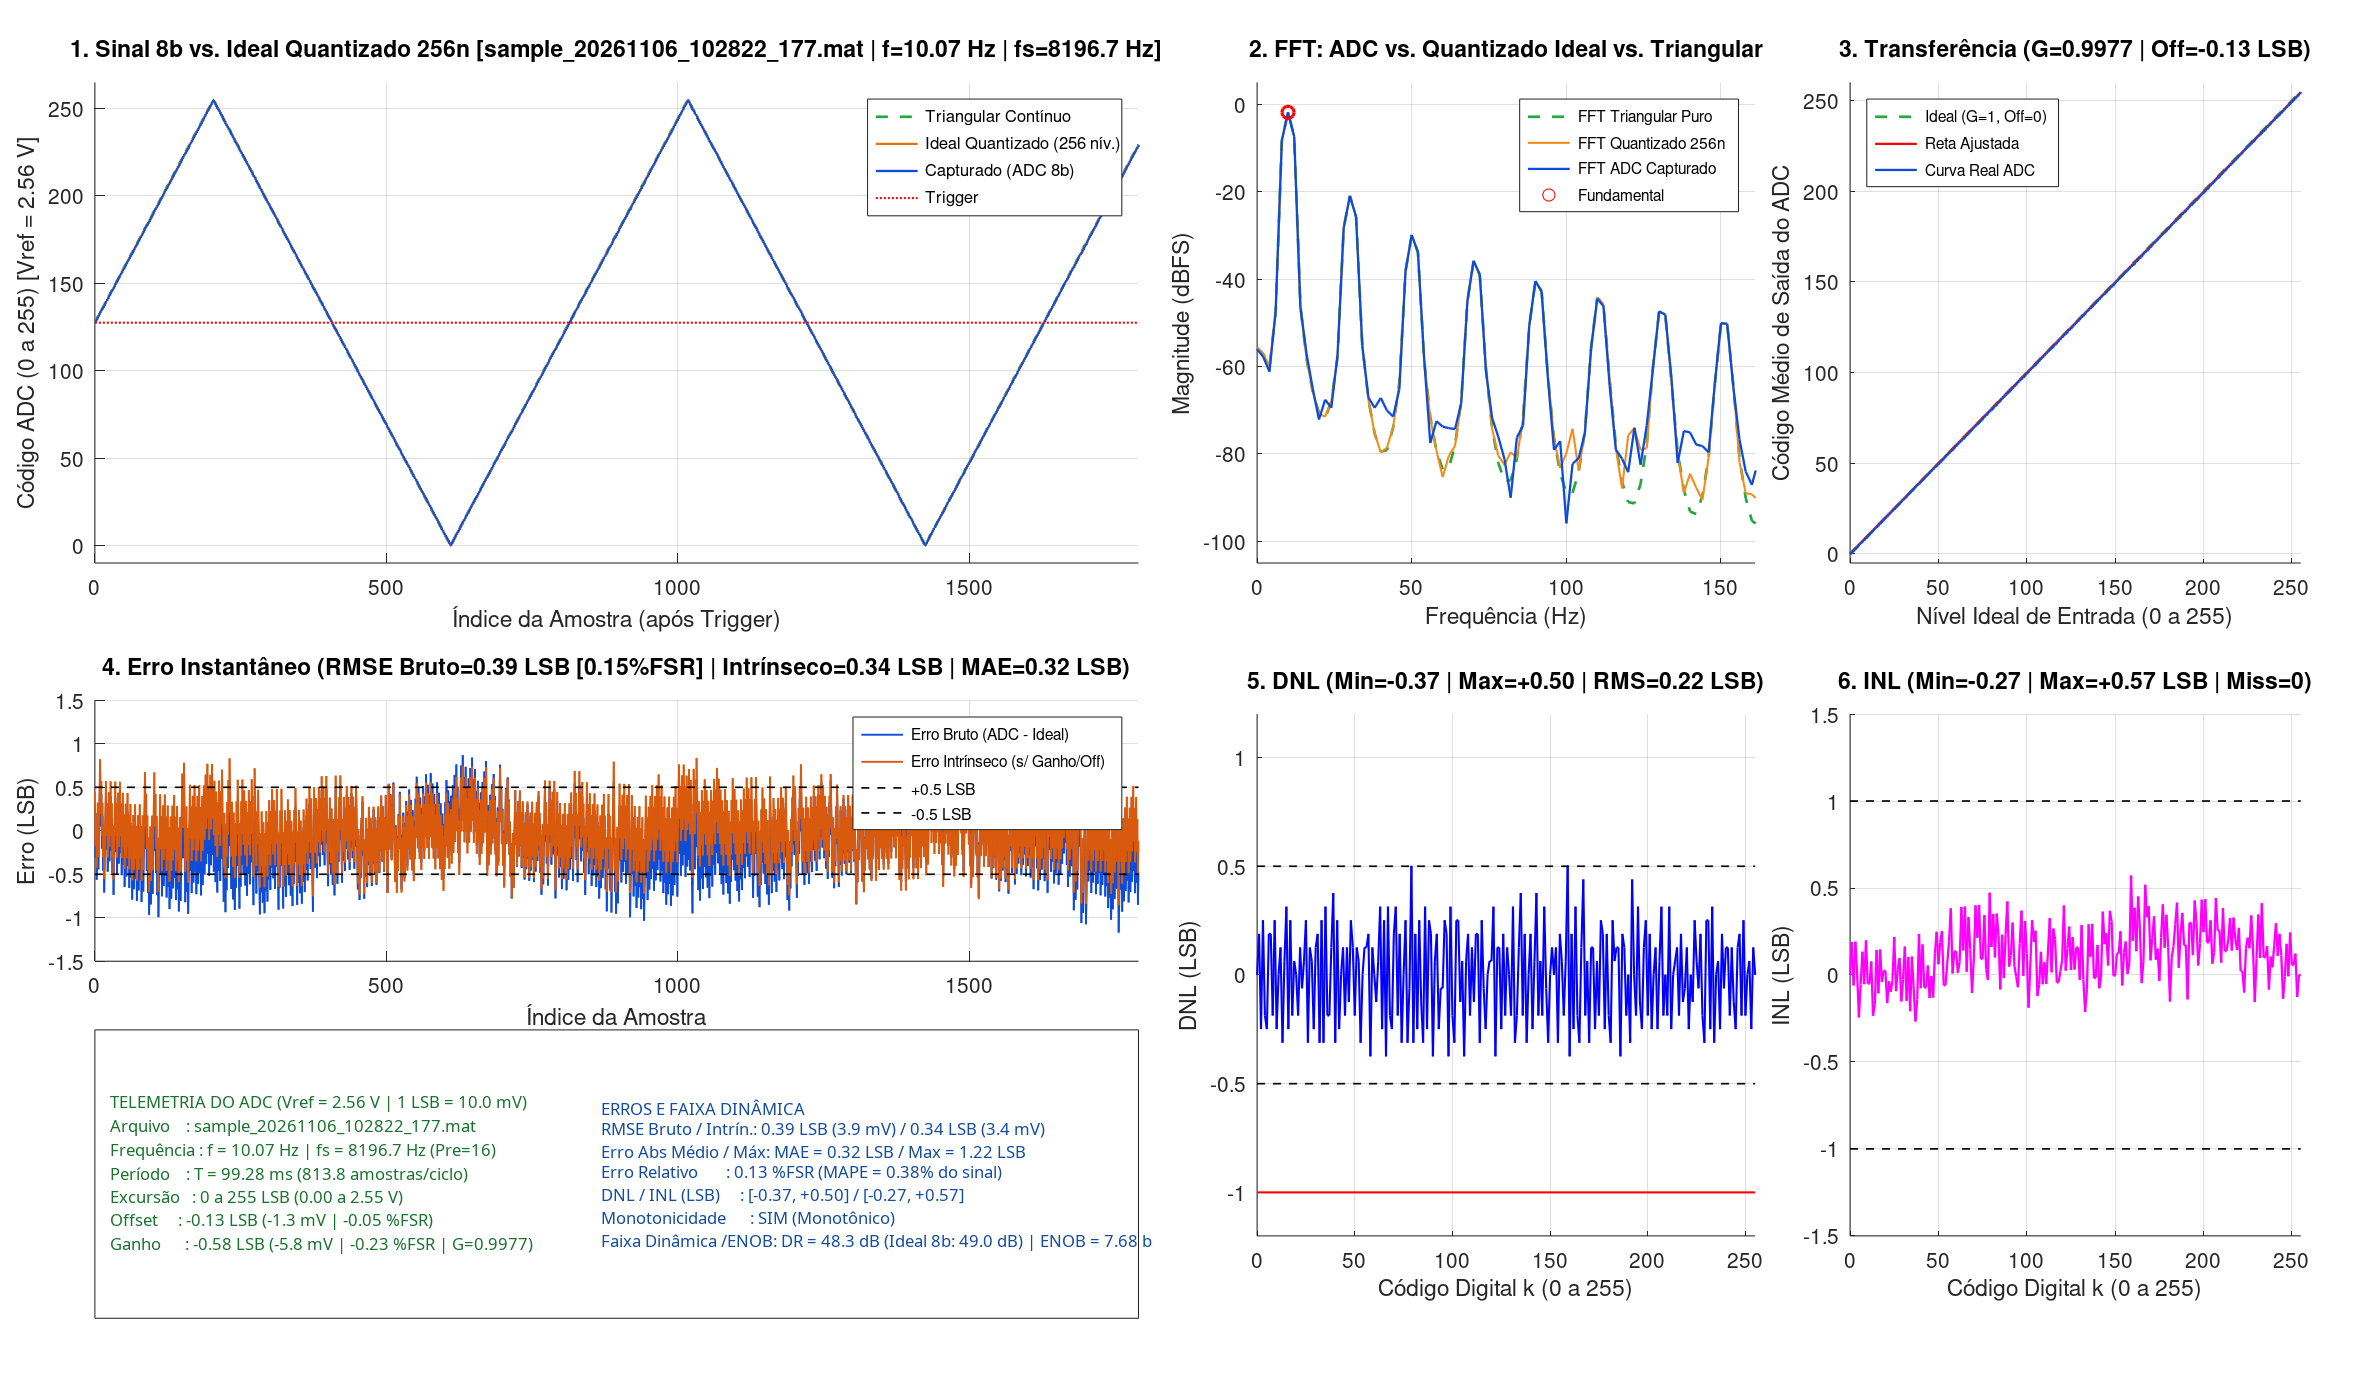
\includegraphics[width=0.98\linewidth,height=6.2cm,keepaspectratio]{Imagens/analysis_10hz.png}\\[2pt]
{\scriptsize \textcolor{structure}{Figura:} Painel completo gerado pelo analisador em GNU Octave para a captura de referência de $10\text{ Hz}$.}
\end{frame}

\begin{frame}{Comparação no Tempo}
\centering
\begin{tikzpicture}
\begin{axis}[
  name=topplot,
  pblplot,
  width=0.94\linewidth,
  height=3.45cm,
  ylabel={Código ADC},
  ylabel style={font=\footnotesize},
  xmin=0,xmax=1750,ymin=-10,ymax=268,
  xticklabel=\empty,
  grid style={gray!25,dashed},
  legend style={at={(0.5,1.05)},anchor=south,legend columns=2,font=\scriptsize,draw=gray!40,fill=gray!5,rounded corners=2pt,/tikz/every even column/.append style={column sep=0.3cm}}
]
\addplot[green!55!black,dashed,line width=1pt] table[x index=0,y index=2]{resultados/tempo_10hz.dat};
\addplot[blue!80!black,const plot,line width=0.7pt,legend image post style={sharp plot}] table[x index=0,y index=1]{resultados/tempo_10hz.dat};
\legend{Triangular ideal ajustada, Leitura do ADC (8 bits)}
\end{axis}

\begin{axis}[
  at={(topplot.south)},
  anchor=north,
  yshift=-0.32cm,
  pblplot,
  width=0.94\linewidth,
  height=2.45cm,
  xlabel={Índice da amostra após trigger ($f = 10{,}072\text{ Hz}$, $f_s = 8196{,}72\text{ Hz}$)},
  ylabel={Erro (LSB)},
  ylabel style={font=\footnotesize},
  xmin=0,xmax=1750,ymin=-1.1,ymax=1.1,
  ytick={-1,-0.5,0,0.5,1},
  grid style={gray!25,dashed}
]
\addplot[blue!75!black, opacity=0.75, line width=0.4pt] table[x index=0,y index=4]{resultados/tempo_10hz.dat};
\addplot[red!80!black,dashed,line width=0.8pt,domain=0:1750] {0.5};
\addplot[red!80!black,dashed,line width=0.8pt,domain=0:1750] {-0.5};
\end{axis}
\end{tikzpicture}
\par\vspace{-0.05cm}\footnotesize \textbf{RMSE bruto:} $0{,}393\text{ LSB}$ \quad$\vert$\quad \textbf{RMSE residual:} $0{,}339\text{ LSB}$ (faixa ideal: $\pm 0{,}5\text{ LSB}$).
\end{frame}

\begin{frame}{Comparação no Domínio da Frequência}
\centering
\begin{tikzpicture}
\begin{axis}[
  pblplot,
  width=0.96\linewidth,
  height=4.8cm,
  xlabel={Frequência (Hz)},
  ylabel={Magnitude (dBFS)},
  xmin=0,xmax=170,ymin=-105,ymax=6,
  xtick={0,10,30,50,70,90,110,130,150,170},
  grid style={gray!25,dashed},
  legend style={at={(0.5,1.04)},anchor=south,legend columns=3,font=\scriptsize,draw=gray!40,fill=gray!5,rounded corners=2pt}
]
\addplot[green!55!black,dashed,line width=1pt] table[x index=0,y index=3]{resultados/fft_10hz.dat};
\addplot[orange!90!black,line width=0.9pt] table[x index=0,y index=2]{resultados/fft_10hz.dat};
\addplot[blue!80!black,line width=0.8pt] table[x index=0,y index=1]{resultados/fft_10hz.dat};
\legend{Triangular contínua, Ideal quantizada (8 bits), Medida no ADC}
\end{axis}
\end{tikzpicture}
\vspace{-0.1cm}
\begin{exampleblock}{Análise espectral ($f_0 \approx 10\text{ Hz}$)}
\footnotesize
\begin{itemize}
\item Picos nas \textbf{harmônicas ímpares} ($10, 30, 50, 70\text{ Hz}\dots$) com decaimento teórico de $1/k^2$, coincidindo com o modelo ideal;
\item Piso de ruído próximo ao limite de quantização de 8 bits (remoção de média DC e janela de Hann).
\end{itemize}
\end{exampleblock}
\end{frame}

\section{Resultados e Discussões}

\begin{frame}{Verificação do Sinal na Bancada}
\begin{columns}[c]
\column{0.46\textwidth}
\centering
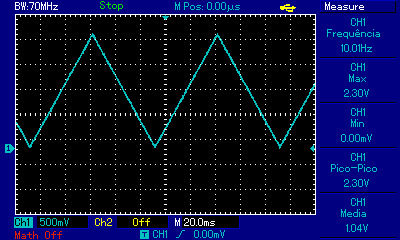
\includegraphics[width=\linewidth,height=3.6cm,keepaspectratio]{Imagens/bancada/10hz_medidas.jpg}\\[2pt]
{\scriptsize \textcolor{structure}{Figura:} Onda triangular ($10\text{ Hz}$) no osciloscópio.}

\column{0.51\textwidth}
\begin{block}{Parâmetros do Sinal ($10\text{ Hz}$)}
\scriptsize
\setlength{\tabcolsep}{4pt}
\renewcommand{\arraystretch}{1.12}
\begin{tabular*}{\linewidth}{@{\extracolsep{\fill}}lrr}
\hline
\textbf{Grandeza} & \textbf{Gerador} & \textbf{Osciloscópio} \\\hline
Frequência ($f$) & $10{,}00\text{ Hz}$ & $10{,}01\text{ Hz}$ \\
Amplitude ($V_{pp}$) & $2{,}270\text{ V}$ & $2{,}30\text{ V}$ \\
Tensão máx. ($V_{\max}$) & $2{,}280\text{ V}$ & $2{,}30\text{ V}$ \\
Tensão mín. ($V_{\min}$) & $0{,}010\text{ V}$ & $0{,}00\text{ V}$ \\
Centro / Offset & $1{,}145\text{ V}$ & $1{,}15\text{ V}$ \\
Média na tela & --- & $1{,}04\text{ V}$ \\\hline
\end{tabular*}
\end{block}
\end{columns}

\vspace{0.15cm}
\begin{exampleblock}{Adequação à faixa real do ADC}
\footnotesize
\begin{itemize}
\item \textbf{Discrepância no $V_{\text{ref}}$ real:} embora a referência interna nominal seja $2{,}56\text{ V}$, o Arduino Mega saturava acima de $2{,}31\text{ V}_{pp}$;
\item \textbf{Ajuste de offset e fundo de escala:} devido ao desvio de offset e ganho do ADC em relação ao sinal medido, ajustou-se o gerador ($2{,}270\text{ V}_{pp}$, offset de $1{,}145\text{ V}$) para enquadrar a excursão entre os códigos $0$ e $255$ sem saturação.
\end{itemize}
\end{exampleblock}
\end{frame}

\subsection{Offset}

\begin{frame}{Caracterização (Offset)}

\begin{columns}

    \column{0.45\linewidth}

    \begin{exampleblock}{Caracterização}
        O erro de offset é caracterizado por um deslocamento constante na curva de conversão do ADC. O erro de offset provoca um deslocamento na resposta do ADC.
    \end{exampleblock}

    \begin{alertblock}{Segundo o Datasheet}
        Sob condição de avaliação do datasheet, o erro típico offset é $-2$ LSB.
    \end{alertblock}

    \column{0.50\linewidth}

    \begin{figure}
        \centering
        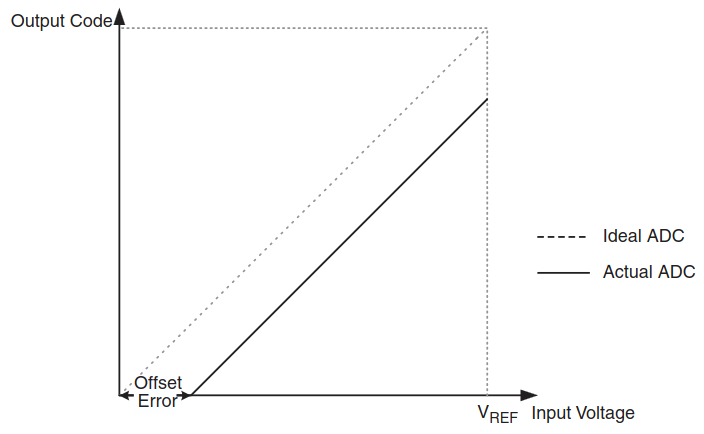
\includegraphics[width=\linewidth]{Imagens/4.png}
        \caption{Caracterização do erro de Offset. Adaptado de: (ATMEL Corporation, 2015).}
        \label{fig4}
    \end{figure}
    
\end{columns}
    
\end{frame}

\begin{frame}{Comparação e Avaliação (Offset)}
\begin{block}{Modelo linear da curva de transferência ($y_{\text{ADC}} \approx G\cdot y_{\text{ideal}} + b$)}
\footnotesize
Ajusta-se uma reta por regressão linear na região central da rampa (sem saturação):
\begin{itemize}
\item $y_{\text{ADC}}$: código medido pelo ADC ($0$ a $255$);\quad $y_{\text{ideal}}$: nível da rampa ideal de referência ($0$ a $255$);
\item $G$: ganho / inclinação da reta ajustada (ideal: $G = 1$);\quad $b$: intercepto na origem (ideal: $b = 0$).
\end{itemize}
\vspace{-0.1cm}
Avaliando o desvio no centro da escala de 8 bits ($y_{\text{ideal}} = 127{,}5$):
\vspace{-0.15cm}
\[
e_{\text{off}} = \underbrace{(G\cdot 127{,}5 + b)}_{\text{valor ajustado no centro}} - \underbrace{127{,}5}_{\text{centro ideal}}.
\]
\vspace{-0.2cm}
\end{block}

\begin{exampleblock}{Resultado Experimental vs. Datasheet ($10\text{ Hz}$)}
\footnotesize
\begin{itemize}
\item \textbf{Captura de referência ($10\text{ Hz}$):} $e_{\text{off}} = \boxed{-0{,}132\text{ LSB}}$ ($\approx -1{,}32\text{ mV}$ na escala de $10\text{ mV/LSB}$);
\item \textbf{Consistência nas 13 capturas ($1\text{ Hz}$ a $60\text{ Hz}$):} variou entre $-0{,}38\text{ LSB}$ e $+0{,}05\text{ LSB}$, bem abaixo do erro típico do datasheet ($\pm 2\text{ LSB}$).
\end{itemize}
\end{exampleblock}
\end{frame}

\subsection{Ganho}

\begin{frame}{Caracterização (Ganho)}

\begin{columns}

    \column{0.45\linewidth}

    \begin{exampleblock}{Caracterização}
        O erro de ganho ocorre quando o conversor apresenta uma variação proporcional entre o valor esperado e o valor efetivamente convertido, isto é, inclinação diferente da ideal na relação entre entrada e saída.
    \end{exampleblock}

    \begin{alertblock}{Segundo o Datasheet}
        \begin{itemize}
            \item
            Sob condição de avaliação do datasheet, o erro típico de ganho é $2$ LSB.
        \end{itemize}
    \end{alertblock}

    \column{0.50\linewidth}

    \begin{figure}
        \centering
        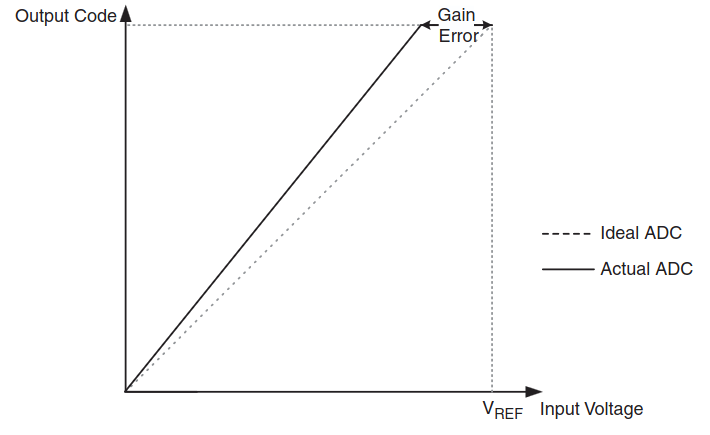
\includegraphics[width=\linewidth]{Imagens/5.png}
        \caption{Caracterização do erro de Ganho. Adaptado de: (ATMEL Corporation, 2015).}
        \label{fig5}
    \end{figure}
    
\end{columns}
    
\end{frame}

\begin{frame}{Comparação e Avaliação (Ganho)}
\begin{block}{Desvio de inclinação no fundo de escala ($y_{\text{ADC}} \approx G\cdot y_{\text{ideal}} + b$)}
\footnotesize
A partir da inclinação $G$ da reta ajustada entre o código medido ($y_{\text{ADC}}$) e a referência ideal ($y_{\text{ideal}}$), o erro de ganho ($e_G$) mede o desvio acumulado de inclinação ao longo de toda a excursão de 8 bits ($255\text{ LSB}$):
\[
e_G = \underbrace{(G - 1)}_{\text{desvio de inclinação}} \cdot \underbrace{255}_{\text{fundo de escala (LSB)}} \implies \text{Para } G = 0{,}99774:\quad e_G = \boxed{-0{,}577\text{ LSB}}.
\]
\end{block}

\begin{columns}[c]
\column{0.47\textwidth}
\begin{block}{Métricas na captura de $10\text{ Hz}$}
\scriptsize
\setlength{\tabcolsep}{4pt}
\renewcommand{\arraystretch}{1.12}
\begin{tabular*}{\linewidth}{@{\extracolsep{\fill}}lr}
\hline
\textbf{Parâmetro} & \textbf{Valor medido}\\\hline
Inclinação ajustada ($G$) & $0{,}99774$\\
Erro de ganho ($e_G$) & $-0{,}577\text{ LSB}$\\
RMSE bruto & $0{,}393\text{ LSB}$\\
RMSE residual (sem $G$/$b$) & $0{,}339\text{ LSB}$\\\hline
\end{tabular*}
\end{block}

\column{0.47\textwidth}
\begin{exampleblock}{Avaliação vs. Datasheet}
\footnotesize
\begin{itemize}
\item $|e_G| = 0{,}577\text{ LSB}$ ($\approx -5{,}77\text{ mV}$), inferior ao típico do datasheet ($2\text{ LSB}$);
\item Ao compensar $G$ e $b$, o RMSE cai de $0{,}393$ para $0{,}339\text{ LSB}$ (próximo do ideal de $0{,}289\text{ LSB}$).
\end{itemize}
\end{exampleblock}
\end{columns}
\end{frame}

\subsection{Não Linearidade Integral (INL)}

\begin{frame}{Caracterização (INL)}

\begin{columns}

    \column{0.45\linewidth}

    \begin{exampleblock}{Caracterização}
        O erro de INL é caracterizado pelo desvio entre a curva real de conversão do dispositivo e a curva ideal de referência.
        A INL representa a máxima diferença entre a resposta real do conversor e a resposta ideal, considerando todos os pontos de conversão.
    \end{exampleblock}

    \begin{alertblock}{Segundo o Datasheet}
        Sob condição de avaliação do datasheet, o erro típico de INL é $1{,}25$ LSB.
    \end{alertblock}

    \column{0.50\linewidth}

    \begin{figure}
        \centering
        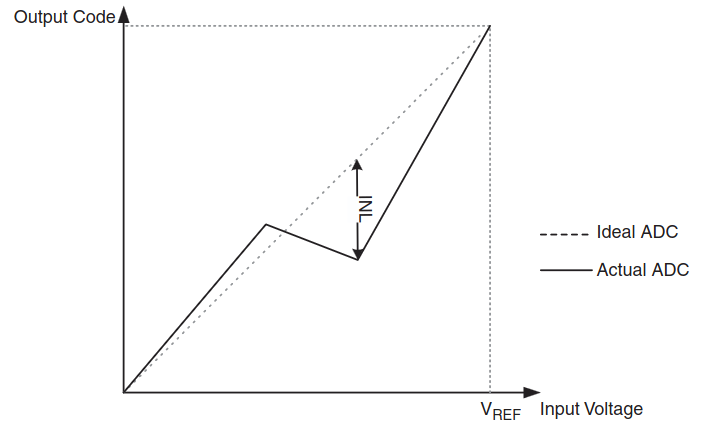
\includegraphics[width=\linewidth]{Imagens/6.png}
        \caption{Caracterização do erro de INL. Adaptado de: (ATMEL Corporation, 2015).}
        \label{fig6}
    \end{figure}
    
\end{columns}
    
\end{frame}

\begin{frame}{Comparação e Avaliação (INL)}
\centering
\begin{tikzpicture}
\begin{axis}[pblplot,height=3.4cm,xlabel={Código ADC ($k$)},ylabel={INL estimada (LSB)},xmin=0,xmax=255,ymin=-0.8,ymax=0.8]
\addplot[magenta,thick] table[x index=0,y index=2]{resultados/linearidade_10hz.dat};
\end{axis}
\end{tikzpicture}

\vspace{-0.15cm}
\begin{exampleblock}{Cálculo Acumulado e Avaliação da INL ($10\text{ Hz}$)}
\footnotesize
Sobre um número inteiro de períodos $N_{\text{int}} = \lfloor N / T_p \rfloor \cdot T_p$, sendo $H(k)$ a contagem do código $k \in \{k_{\min}+1, \dots, k_{\max}-1\}$ e $\overline{H}$ a contagem média esperada por nível:
\vspace{-0.15cm}
\[
\text{INL}(k) = \sum_{j=k_{\min}+1}^{k} \left[\text{DNL}(j) - \overline{\text{DNL}}\right] \qquad \left(\text{Excursão: } [-0{,}27;\ +0{,}57]\text{ LSB} < 1{,}25\text{ LSB}\right).
\]
\vspace{-0.25cm}
\end{exampleblock}
\end{frame}

\subsection{Não Linearidade Diferencial (DNL)}

\begin{frame}{Caracterização (DNL)}

\begin{columns}

    \column{0.45\linewidth}

    \begin{exampleblock}{Caracterização}
        O erro de DNL é caracterizado pela diferença entre o tamanho real de cada intervalo de conversão e o tamanho ideal.
    \end{exampleblock}

    \begin{alertblock}{Avaliação de DNL}
        \begin{itemize}
            \item DNL = 0;
            \item DNL positivo;
            \item DNL negativo;
            \item DNL = $-1$ LSB;
            \item Sob condição de avaliação do datasheet, o erro típico de DNL é $0{,}5$ LSB.
        \end{itemize}
    \end{alertblock}

    \column{0.50\linewidth}

    \begin{figure}
        \centering
        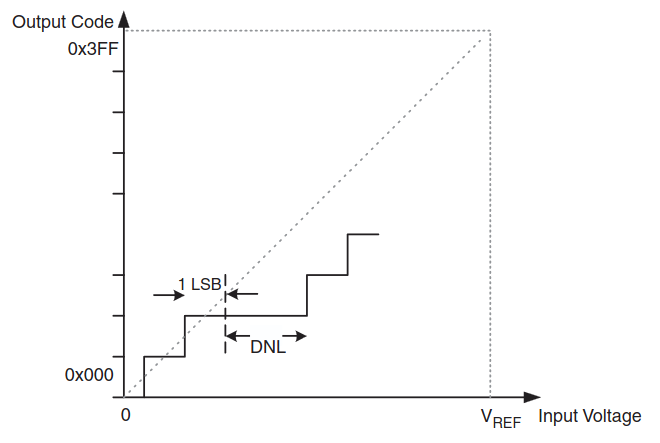
\includegraphics[width=\linewidth]{Imagens/7.png}
        \caption{Caracterização do erro de DNL. Adaptado de: (ATMEL Corporation, 2015).}
        \label{fig7}
    \end{figure}
    
\end{columns}
    
\end{frame}

\begin{frame}{Comparação e Avaliação (DNL)}
\centering
\begin{tikzpicture}
\begin{axis}[pblplot,height=3.3cm,xlabel={Código ADC ($k$)},ylabel={DNL estimada (LSB)},xmin=0,xmax=255,ymin=-1.05,ymax=0.8]
\addplot[blue] table[x index=0,y index=1]{resultados/linearidade_10hz.dat};
\addplot[red,dashed,thick,domain=0:255] {-1};
\end{axis}
\end{tikzpicture}

\vspace{-0.15cm}
\begin{exampleblock}{Avaliação de DNL e Ausência de Códigos Faltantes (\textit{Missing Codes})}
\footnotesize
\[
\text{DNL}(k) = \frac{H(k)}{\overline{H}} - 1 \qquad \left(\text{Excursão medida em } 10\text{ Hz: } [-0{,}37;\ +0{,}50]\text{ LSB}\right)
\]
\vspace{-0.25cm}
\begin{itemize}
    \item \textbf{Importância de não haver códigos faltantes} (\textit{missing codes})\textbf{:} se $\text{DNL}(k) = -1{,}0\text{ LSB}$ ($H(k) = 0$, linha vermelha tracejada), o código $k$ jamais é produzido pelo conversor, perdendo informação;
    \item \textbf{Monotonicidade garantida:} como $\text{DNL}(k) > -1{,}0\text{ LSB}$ em todos os níveis ($0$ \textit{missing codes}) e $\Delta \overline{y}_{\text{ADC}}(k) \ge 0$, o conversor é estritamente monotônico em toda a escala.
\end{itemize}
\end{exampleblock}
\end{frame}

\section{Considerações Finais}

\begin{frame}{Síntese dos Resultados e Considerações Finais}
\begin{block}{Resultados nas Capturas de Referência (Erros em LSB)}
\scriptsize
\setlength{\tabcolsep}{3pt}
\renewcommand{\arraystretch}{1.08}
\begin{tabular*}{\linewidth}{@{\extracolsep{\fill}}rrrrrc}
\hline
\textbf{$f$ (Hz)} & \textbf{$f_s$ (Hz)} & \textbf{DNL [mín; máx]} & \textbf{INL [mín; máx]} & \textbf{RMSE} & \textbf{Monotônico} \\\hline
$1{,}006$ & $1024{,}1$ & $[-0{,}43;\ +0{,}52]$ & $[-0{,}45;\ +0{,}38]$ & $0{,}350$ & Sim \\
$5{,}032$ & $4000{,}0$ & $[-0{,}48;\ +0{,}49]$ & $[-0{,}32;\ +0{,}50]$ & $0{,}353$ & Sim \\
$8{,}066$ & $8196{,}7$ & $[-0{,}49;\ +0{,}59]$ & $[-0{,}40;\ +0{,}53]$ & $0{,}364$ & Sim \\
$\mathbf{10{,}072}$ & $\mathbf{8196{,}7}$ & $\mathbf{[-0{,}37;\ +0{,}50]}$ & $\mathbf{[-0{,}27;\ +0{,}57]}$ & $\mathbf{0{,}339}$ & \textbf{Sim} \\
$30{,}246$ & $16\,393{,}4$ & $[-0{,}52;\ +0{,}50]$ & $[-0{,}22;\ +0{,}62]$ & $0{,}337$ & Sim \\
$60{,}491$ & $32\,786{,}9$ & $[-0{,}66;\ +0{,}77]$ & $[-0{,}45;\ +0{,}63]$ & $0{,}347$ & Sim \\\hline
\end{tabular*}
\end{block}

\vspace{-0.15cm}
\begin{exampleblock}{Considerações Finais}
\footnotesize
\begin{itemize}
\item \textbf{Desempenho do ADC:} Conversão monotônica em toda a faixa ($1$ a $60\text{ Hz}$), sem \textit{missing codes} e com INL, DNL e RMSE compatíveis com o datasheet;
\item \textbf{Arquitetura de Captura:} O buffer em RAM ($4096\text{ amostras}$) com envio UART pós-captura garantiu amostragem determinística até $f_{s,\max} = 32\,786{,}9\text{ Hz}$;
\item \textbf{Critérios de Ensaio:} O ajuste à faixa real do $V_{\text{ref}}$ e a relação $512 \le f_s/f \le 4096$ evitaram saturação, subamostragem por rampa e truncamento de ciclo.
\end{itemize}
\end{exampleblock}
\end{frame}

\section{Referências}

\begin{frame}{Referências}
    \footnotesize

    \begin{thebibliography}{99}

    \bibitem{oppenheim-sinais}
    OPPENHEIM, Alan V.; WILLSKY, Alan S.; NAWAB, S. Hamid.
    \textit{Sinais e sistemas}.
    2. ed. São Paulo: Pearson Prentice Hall, 2010.

    \bibitem{oppenheim-processamento}
    OPPENHEIM, Alan V.; SCHAFER, Ronald W.; BUCK, John R.
    \textit{Processamento em tempo discreto de sinais}.
    2. ed. São Paulo: Pearson Prentice Hall, 2009.

    \bibitem{allaboutcircuits}
    Elliott Smith.
    \textit{Understanding the Successive Approximation Register ADC}.
    Disponível em:
    \url{https://www.allaboutcircuits.com/technical-articles/understanding-analog-to-digital-converters-the-successive-approximation-reg/}.
    Acesso em: 1 nov. 2026.

    \bibitem{atmega2560} ATMEL Corporation. \textit{ATmega2560: 8-bit Microcontroller with 256K Bytes In-System Programmable Flash}. Disponível em: \url{https://www.alldatasheet.com/datasheet-pdf/view/107092/ATMEL/ATMEGA2560.html}. Acesso em: 4 nov. 2026.

    \end{thebibliography}
\end{frame}

\end{document}